% \subsection{Ejercicio 3 - Secuencia de cuatro LEDs}\label{subsec:ej3}

Como en el ejercicio anterior, hay que indicar que la página sea apaisada (\myref{fun:pghorizontal}).\\

Para dibujar el corazón se usan dos semicírculos (de 0 hasta 180 grados) y un triángulo (pirámide invertida):
\begin{lstlisting}[language=PostScript, caption=Corazón, captionpos=b, label=fun:corazon]
 % Parte izquierda
newpath
    1 0 0 setrgbcolor  % Color rojo
    3 setlinewidth
    200 300 60 0 180 arc  
    fill
stroke

% Parte derecha
newpath 
    1 0 0 setrgbcolor  % Color rojo
    320 300 60 0 180 arc   
    fill
stroke

% Pico (triángulo)
newpath 
    1 0 0 setrgbcolor  % Color rojo
    140 300 moveto % Esquina superior izquierda
    240 0 rlineto   % Línea hacia la derecha
    -120 -120 rlineto   % Línea hacia abajo-izq
    closepath 
    fill
stroke
\end{lstlisting}

Además, para la poesía se usa la función \textit{show} y con la función \textit{setrgbcolor} se crean distintos tonos de azul jugando con la componente $G$ y $B$.\\

\begin{lstlisting}[language=PostScript, caption=Poesía, captionpos=b, label=fun:poesia]
/Times-Italic findfont 18 scalefont setfont % Fuente
newpath
    0 0.2 1 setrgbcolor  % Azul oscuro
    450 300 moveto 
    (Dale limosna, mujer,) show

    0 0.4 1 setrgbcolor  % Azul medio
    450 280 moveto 
    (que no hay en la vida nada,) show

    0 0.6 1 setrgbcolor  % Azul claro
    450 260 moveto 
    (como la pena de ser) show

    0 0.8 1 setrgbcolor  % Azul muy claro
    450 240 moveto 
    (ciego en Granada.) show

    0 0.1 0.5 setrgbcolor % Contraste para el autor
    470 220 moveto 
    (Francisco de Icaza.) show
stroke
showpage
\end{lstlisting}
A continuación se muestra la imagen obtenida\myref{fig:3ejer}:
\begin{figure}[H]
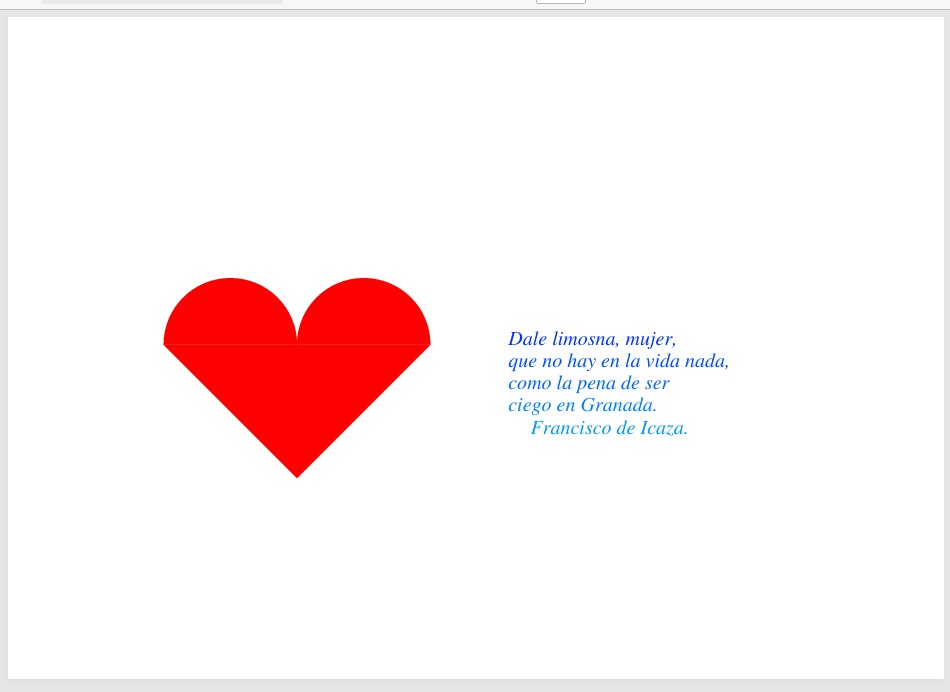
\includegraphics[width=0.9\textwidth]{images/ejer3.jpg}
\caption{Propuesta ejercicio 3.}
\label{fig:3ejer}
\end{figure}

El código completo se puede ver en el anexo \ref{anexo:ej3}. En el anexo \ref{anexo:pdf3} se puede ver la página pdf generada.